% !TEX root = Entwurf_goApp.tex
\section{Sequenzdiagramme}

\subsection{Benutzer zur einer Gruppe hinzufügen}
Im Folgenden werden wir anhand einer Beispiel Funktionalität der goApp interne Abläufe vorstellen.
Im Beispiel geht es darum einen Benutzer der zuvor eine Beitrittsanfrage an eine Gruppe gestellt hat in die Gruppe aufzunehmen.
Hierzu muss der Gründer der Gruppe von der Startseite (StartActivity) zur Gruppeninformationsansicht (GroupInfoActivity) navigieren und dort mit einem Klick die Anfrage bestätigen.
Innerhalb der Datenbank muss hierfür der anfragende Benutzer in die Gruppe hinzugefügt werden und die Beitrittsanfrage anschließend gelöscht werden.
\ \\
\ \\
\ \\
\begin {center}
\makebox[0pt]{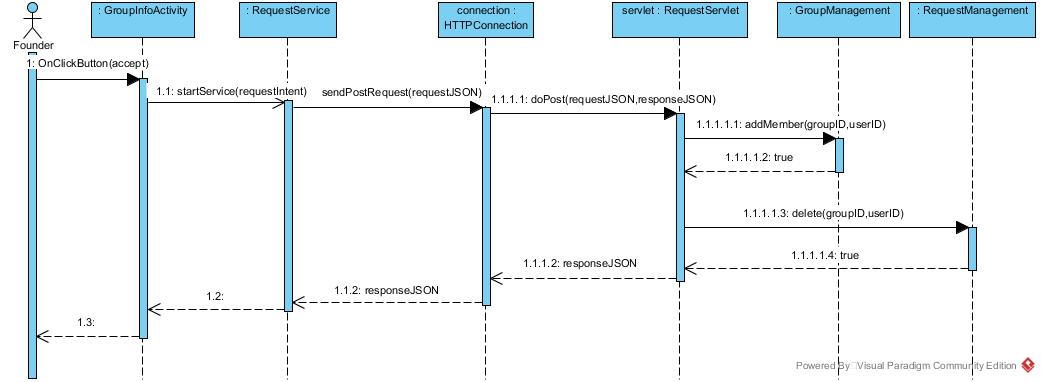
\includegraphics[width=\paperwidth]{addMemberSequenceDiagram.jpg}}
\end {center}
\ \\
\ \\
Obiges Diagramm veranschaulicht grob wie diese Funktionalität in unserer App umgesetzt wird.
Der Gruppengründer befindet sich hier schon in der GroupInfoActivity und drückt dort den Button um die Anfrage anzunehmen.
Die GroupInfoActivity startet daraufhin mit einem Intent den RequestService, welcher sich um jegliche Bearbeitung von Anfragen kümmert.
Der RequestService schickt mithilfe der Klasse HTTPConnection die Anfrage an das RequestServlet, welches das Gegenstück zum RequestService auf dem Server darstellt.
Die Anfrage wird hier ausgewertet und mithilfe der Klassen, welche für die Datenbankverwaltung zuständig sind, umgesetzt. In diesem Fall fügt die Klasse GroupManagement den Benutzer in die Gruppe hinzu und die Klasse RequestManagement löscht die Anfrage, da diese nicht mehr benötigt wird.
Das RequestServlet antwortet daraufhin dem Clienten und der RequestService sorgt dafür, dass der Benutzer über die View ein Feedback bekommt. \newline
Dieses Diagramm zeigt nicht alle Feinheiten der internen Abläufe sondern vereinfacht vieles. Es eignet sich aber um einen ersten Überblick zu erhalten.
Die folgenden Diagramme, Activity-Service Kommunikation, Service-ServerConnection Kommunikation und Servlet-Datenbankmanagement Kommunikation illustrieren deshalb die selbe Anfrage, einen Benutzer der zuvor eine Beitrittsanfrage an eine Gruppe gestellt hat in die Gruppe aufzunehmen, detaillierter und spezifisch auf die jeweilige Kommunikation.

\subsubsection{Activity-Service Kommunikation}

\begin {center}
\makebox[0pt]{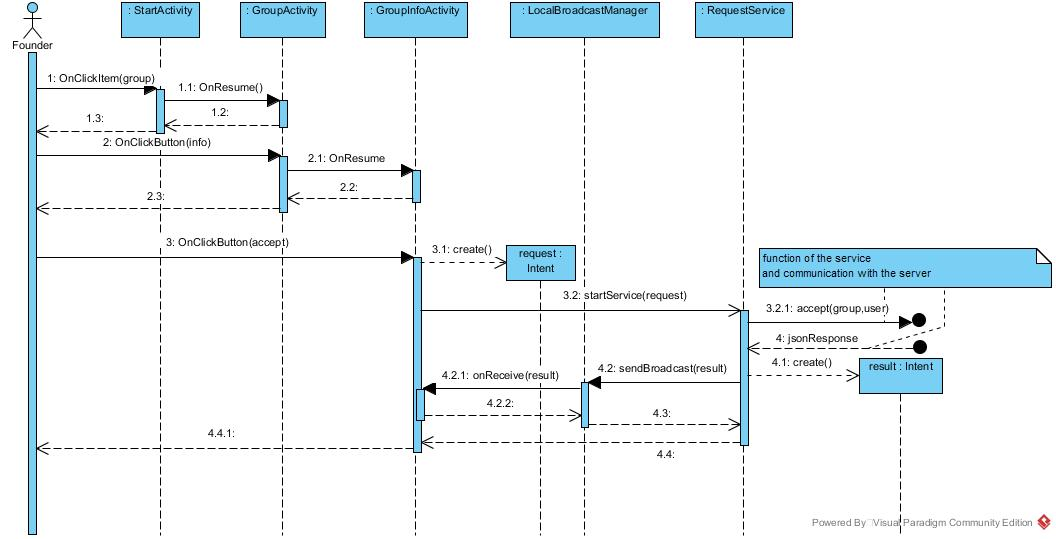
\includegraphics[width=\paperwidth]{Activity_Service.jpg}}
\end {center}
	Wenn der Gruppengründer auf die Gruppe klickt, wechselt die Ansicht zu der GroupActivity. Dort klickt er auf Info was ihn zur GroupInfoActivity führt. Bei dieser werden ihm alle Gruppenanfragen angezeigt. Da er den Anfragesteller zur Gruppe  hinzufügen will klickt er auf Anfrage annehmen. Dadurch wird die Methode OnClickButton der GroupInfoActivity aufgerufen. Diese erstellt einen Intent in dem enthalten ist, welche Methode des Services ausgeführt werden soll und die dafür nötigen Parameter. 
Dieser Intent wird dann bei der Methode startService an den RequestService übergeben. Dieser stellt eine Anfrage an den Server (\hyperlink{ServiceServerConnection}{siehe Service-ServerConnection Kommunikation}). Und erstellt einen Intent in dem die Informationen, die die Activty benötigt stehen. In diesem Fall also ob auf dem Server ein Fehler aufgetreten ist.
Der Intent wird über den LocalBroadcastManager des Andoidsystems an alle registrierten Klassen der App gesendet. Dadurch empfängt die GroupInfoActivity den Intent und kann die Benutzeroberfläche aktualisieren.


\hypertarget{ServiceServerConnection}{}
\subsubsection{Service-ServerConnection Kommunikation}
\begin {center}
\makebox[0pt]{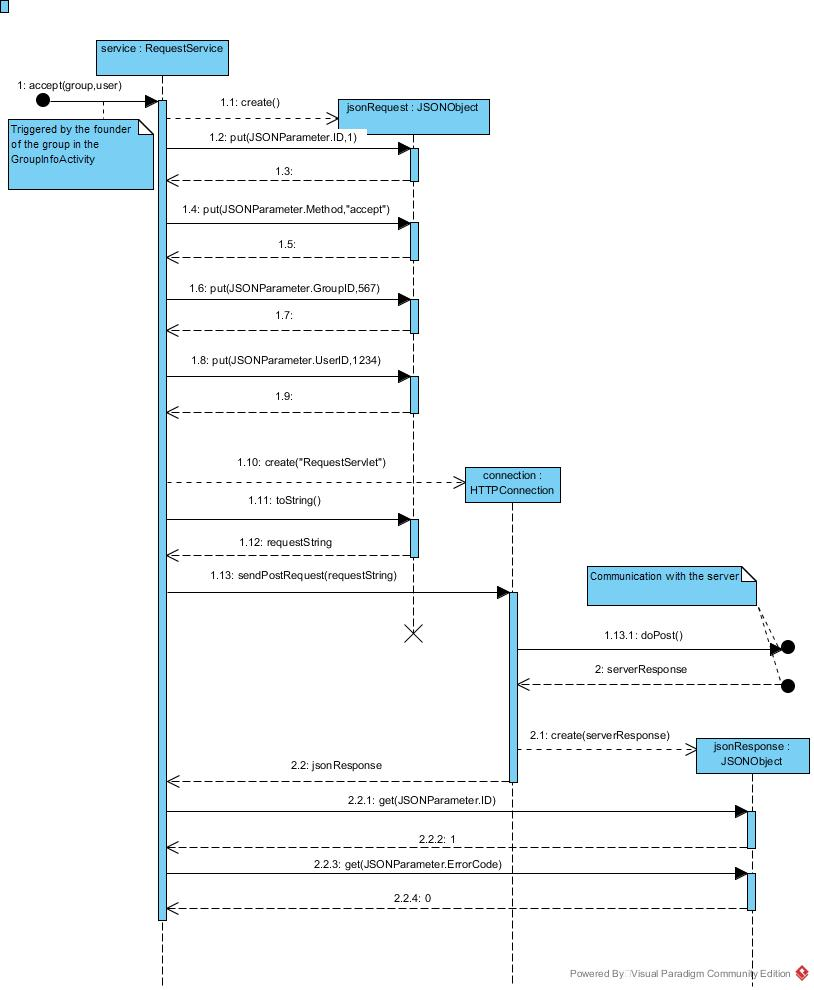
\includegraphics[width=0.9\paperwidth]{Service_ServerConnection.jpg}}
\end {center}

Wenn bei dem RequestService die accept Methode aufgerufen wird, erstellt dieser zunächst ein JSONObject, in dem die Serveranfrage codiert wird. Er fügt dem JSONObject
\begin{itemize}
\item  die ID der Anfrage,
\item den Namen der Methode, welche auf dem Servlet aufgerufen werden soll,
\item die ID der Gruppe, zu der die Gruppenanfrage gehört und
\item die ID des Users welcher in die Gruppe aufgenommen werden will hinzu.
\end{itemize}
Zusätzlich erstellt der Service eine HTTPConnection und übergibt ihr den Namen des Servlets, an welches die Anfrage geschickt werden soll.
Danach holt er sich von dem JSONObject den JSON-String, in dem die zuvor hinzugefügten Daten enthalten sind. Den übergibt er der Methode sendPostRequest des Klasse HTTPConnection.
Diese sendet dann die Anfrage an den Server, welcher die Anfrage bearbeitet (\hyperlink{ServletDatenbank}{siehe Servlet-Datenbankmanagement Kommunikation}). Der Server sendet ein JSON-String als Antwort zurück, aus welchem die sendPostRequest-Methode ein JSONObject erzeugt und dieses an den RequestService zurück gibt. Der RequestService holt sich dann den Error code aus dem JSONObject um zu erkennen ob ein Fehler auftrat und informiert die Activity.



%Der RequestService erstellt daraufhin einen JSONString und leitet diesen an die Klasse %HTTPConnection weiter, diese Klasse liegt im  Package serverConnection und ist der einzige %Kommunikationsweg der App mit dem Server.
%HTTPConnection wählt das Request Servlet aus und startet auf diesem die passende Methode.
%Von hier werden
\hypertarget{ServletDatenbank}{}
\subsubsection{Servlet-Datenbankmanagement Kommunikation}
\begin {center}
\makebox[0pt]{\includegraphics[width=\paperwidth]{Servlet_MAnagement.jpg}}
\end {center}
Wenn bei einem Servlet die doPost Methode aufgerufen wird, erstellt es ein JSONObject zu dem übergebenen JSON-String.
Von diesem holt es sich den Namen der Methode und ruft die entsprechende Methode mit dem JSONObject als Parameter bei sich auf. Die accept-Methode liest dann aus dem JSONObject die GroupId und die UserId aus und erstellt ein GroupManagement Objekt.
Nun ruft das Servlet die addMember-Methode von dem GroupManagement auf. Diese Methode fügt in den User zur Gruppe hinzu. Zusätzlich erstellt das Servlet ein RequestManagement Objekt, bei welchem es die Methode delete aufruft. Diese löscht die Gruppenanfrage aus der Datenbank. Die accept-Methode erstellt dann ein JSONObject und fügt ihm eine AnfrageId und einen ErrorCode, welcher angibt ob ein Fehler auftrat, hinzu. Danach erstellt die Methode den JSON-String aus dem JSONObject und gibt diesen an die doPost-Methode zurück. Diese sendet den JSON-String zurück an den Client.

\subsection{Clusterbildung von Standorten}


\begin {center}
\makebox[0pt]{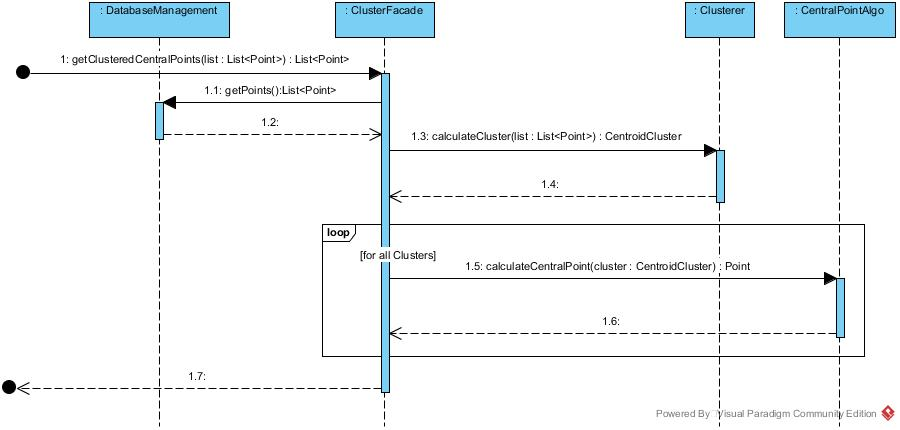
\includegraphics[width=\paperwidth]{AlgorithmSequence.jpg}}
\end {center}

In diesem Kapitel wird die Funktionsweise des Clusteralgorithmuspakets anhand eines Sequenzdiagrammes veranschaulicht. Dabei erhält die Klasse ClusterFacade, die auch als Fassade des Paketes fungiert, einen Aufruf der Methode getClusteredCentralPoints. Hierbei wird das gewünschte Event als Parameter übergeben, dessen zugehörige Daten verarbeitet werden sollen. Hierzu spricht die Klasse ClusterFacade die Klasse DatabaseManagement an, die alle dem Event zugehörige Standorte zurückgibt. Nachfolgend ruft die ClusterFacade Klasse den Clusterer auf, wobei es irrelevant ist um welchen Clusteralgorithmus es sich dabei handelt, sobald er von der Klasse Clusterer erbt. Dem Clusterer werden alle Standorte als Liste von Punkten übergeben, die der Clusterer nun nach jeweiligem Algorithmus clustert. Die geclusterten Punkte werden der Klasse ClusterFacade als Liste an CentroidCluster, eine Clusterstruktur mit explizitem mittleren Punkt, zurückgegeben. Danach ruft ClusterFacade für jedes CentroidCluster der Liste die Methode getCentralPoint der Klasse CentralPointAlgo auf. Die jeweilige Realisierung der abstrakten Klasse CentralPointAlgo berechnet den Kernpunkt des übergebenen Clusters und gibt diesen zurück. ClusterFacade speichert die Kernpunkte in einer Liste und gibt diese letztlich an den Aufrufer der Methode getClusteredCentralPoints zurück. 
	
	\newpage
